A system would be useless if it did not operate according to specification.
Therefore, the platform has been thourougly verified through functional tests, performance analysis and example programs.

%==============================================================================%

\section{Functional Tests}

The functionality of the platform has been verified under normal use conditions with the tests described in Appendix~\ref{app:test-descriptions}.
Each test has a short description and a list of the instructions that are verified given it passes.
Together, the 11 tests cover all system functionality except for fitness, which is designed to be application specific.
The tests are implemented as separate programs, but use a shared test framework.
A full system reset is performed before each test.

All tests are passed for all configurations of the platform that have been implemented, which includes 5x5, 16x16, 32x32, 4x4x4, 8x8x4, 8x8x8, 8x16x4 and 10x10x8 matrix sizes; 5, 6 and 8 type bits; 2, 4, 6, 7 and 8 rules tested in parallel; and 1, 2, 4 and 8 LUT configuration bits.
This proves that the platform is functional and scalable.

\subsection{DFT}

Although the fitness modules have no test programs, the DFT module and the DSP wrapper has their own test benches to ensure that refactoring has not changed functionality.

Testing shows that the DFT produces slightly different output than before.
This is likely due differences is rounding or expression structures between the VHDL and python implementations for generating the twiddle factors.
However, compared to the output of numpy's real fft, the new module is about as precise as the previous.

\todo{DFT test results with standard variation / percentage error}

%==============================================================================%

\section{Example Replicator}

As a proof of concept, the example in \figurename~\ref{fig:replicator} was created to showcase how development can be used to create simple self-replicating structures in a 2D CA that can grow to any desirable size given enough time.
It was manually designed using 17 development rules and 13 cell types, and the source code is available in \textbf{programs/demo\_replicator.c}.

In essence, green cells creates copies of themselves going around in clockwise loops, while cyan cells shoot off from the corners to begin the creation of new loops.
When loops are completed, the center cells turns red.
After the entire structure has formed, the next step would be to use it for computation by specifying LUTs for each cell type.
However, that is outside the scope of this simple example.

\begin{figure}[!ht]
    \centering
    \begin{subfigure}{0.32\textwidth}
        \centering
        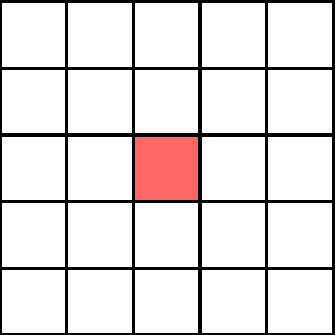
\includegraphics[width=0.9\textwidth]{replicator/00}
        \caption{Step 0}
    \end{subfigure}
    \begin{subfigure}{0.32\textwidth}
        \centering
        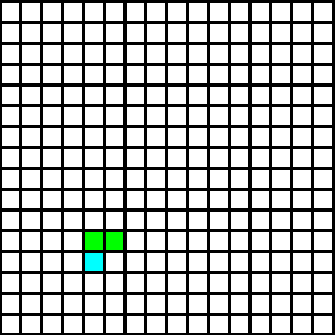
\includegraphics[width=0.9\textwidth]{replicator/01}
        \caption{Step 1}
    \end{subfigure}
    \begin{subfigure}{0.32\textwidth}
        \centering
        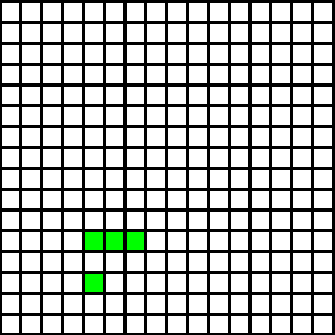
\includegraphics[width=0.9\textwidth]{replicator/02}
        \caption{Step 2}
    \end{subfigure}
    \par\bigskip
    \begin{subfigure}{0.32\textwidth}
        \centering
        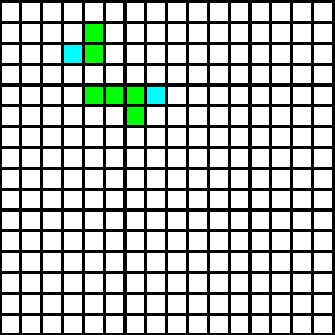
\includegraphics[width=0.9\textwidth]{replicator/03}
        \caption{Step 3}
    \end{subfigure}
    \begin{subfigure}{0.32\textwidth}
        \centering
        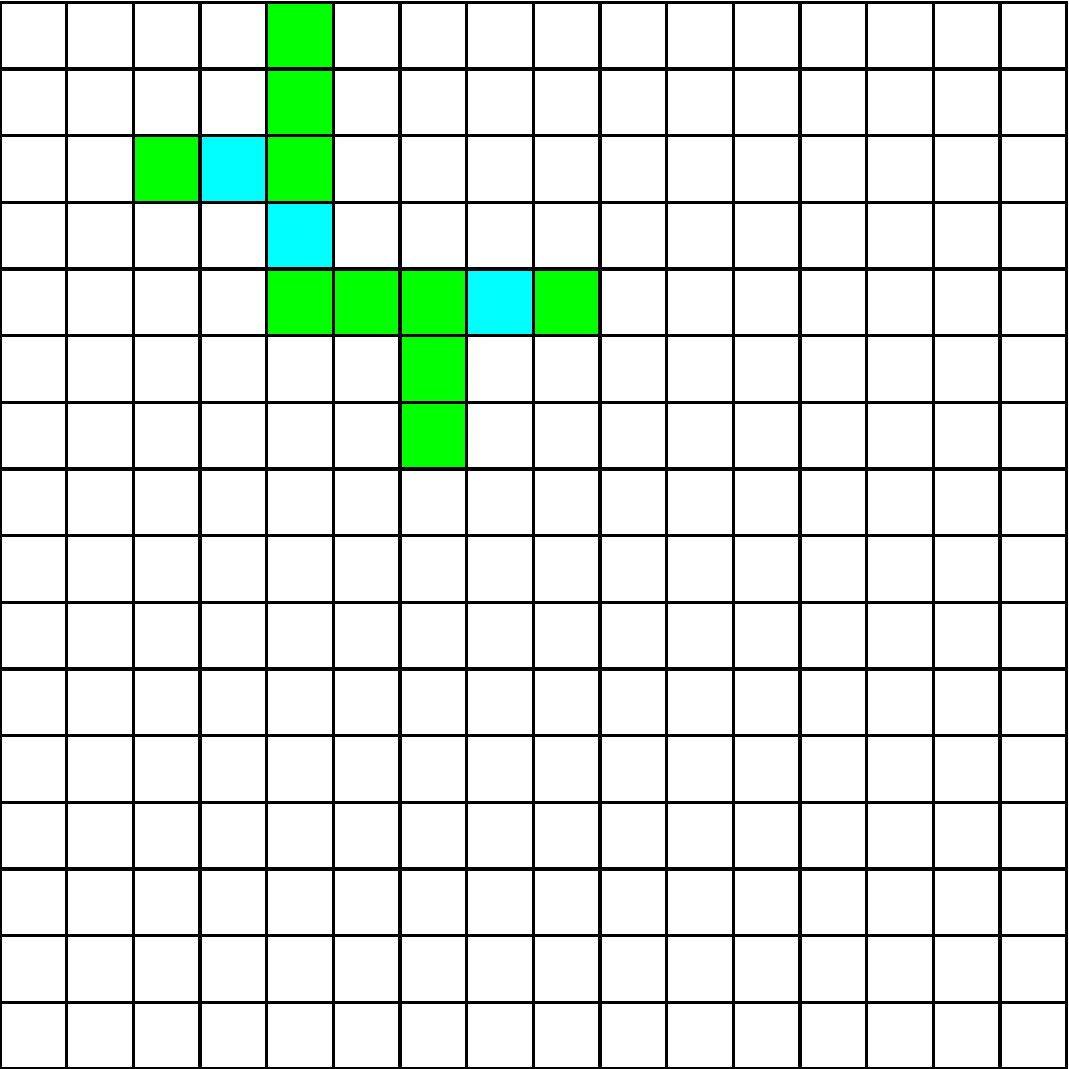
\includegraphics[width=0.9\textwidth]{replicator/04}
        \caption{Step 4}
    \end{subfigure}
    \begin{subfigure}{0.32\textwidth}
        \centering
        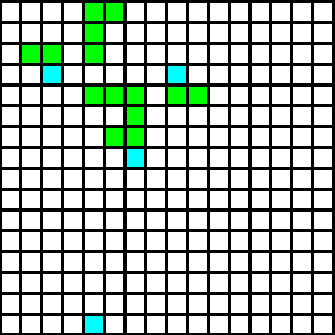
\includegraphics[width=0.9\textwidth]{replicator/05}
        \caption{Step 5}
    \end{subfigure}
    \par\bigskip
    \begin{subfigure}{0.32\textwidth}
        \centering
        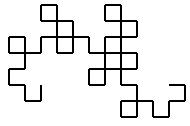
\includegraphics[width=0.9\textwidth]{replicator/06}
        \caption{Step 6}
    \end{subfigure}
    \begin{subfigure}{0.32\textwidth}
        \centering
        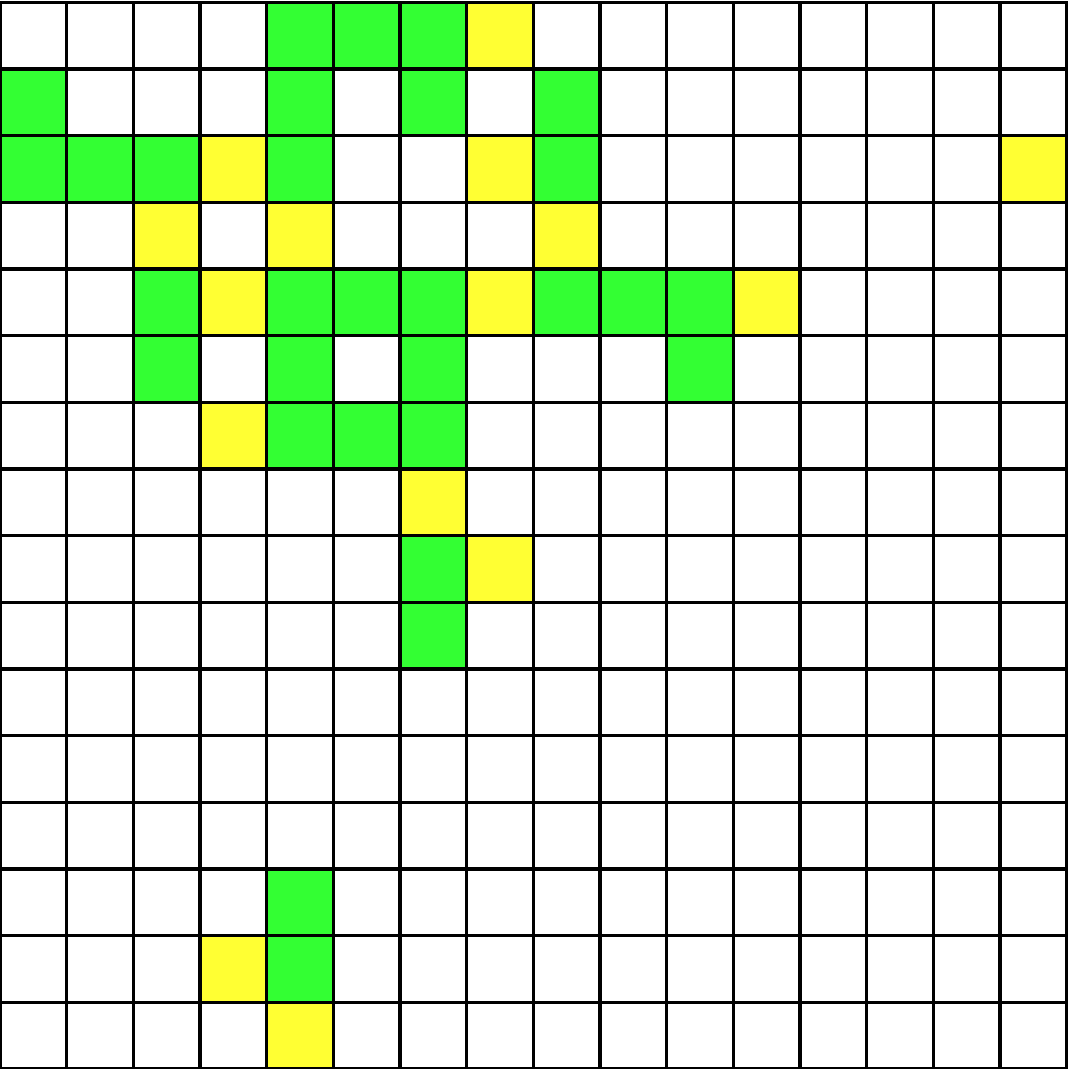
\includegraphics[width=0.9\textwidth]{replicator/07}
        \caption{Step 7}
    \end{subfigure}
    \begin{subfigure}{0.32\textwidth}
        \centering
        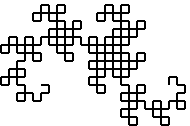
\includegraphics[width=0.9\textwidth]{replicator/08}
        \caption{Step 8}
    \end{subfigure}
    \par\bigskip
    \begin{subfigure}{0.32\textwidth}
        \centering
        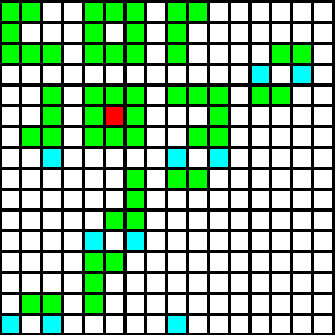
\includegraphics[width=0.9\textwidth]{replicator/09}
        \caption{Step 9}
    \end{subfigure}
    \begin{subfigure}{0.32\textwidth}
        \centering
        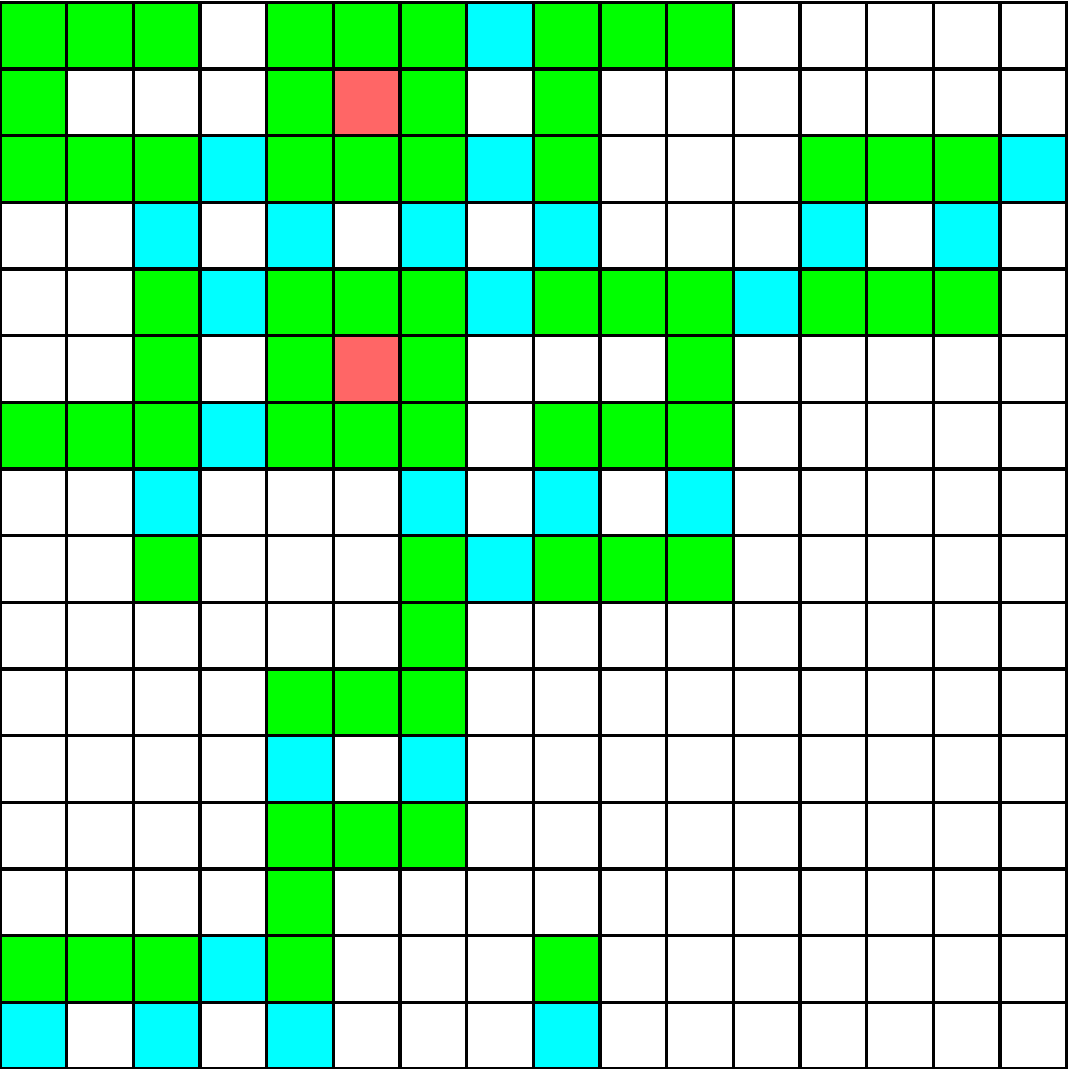
\includegraphics[width=0.9\textwidth]{replicator/10}
        \caption{Step 10}
    \end{subfigure}
    \begin{subfigure}{0.32\textwidth}
        \centering
        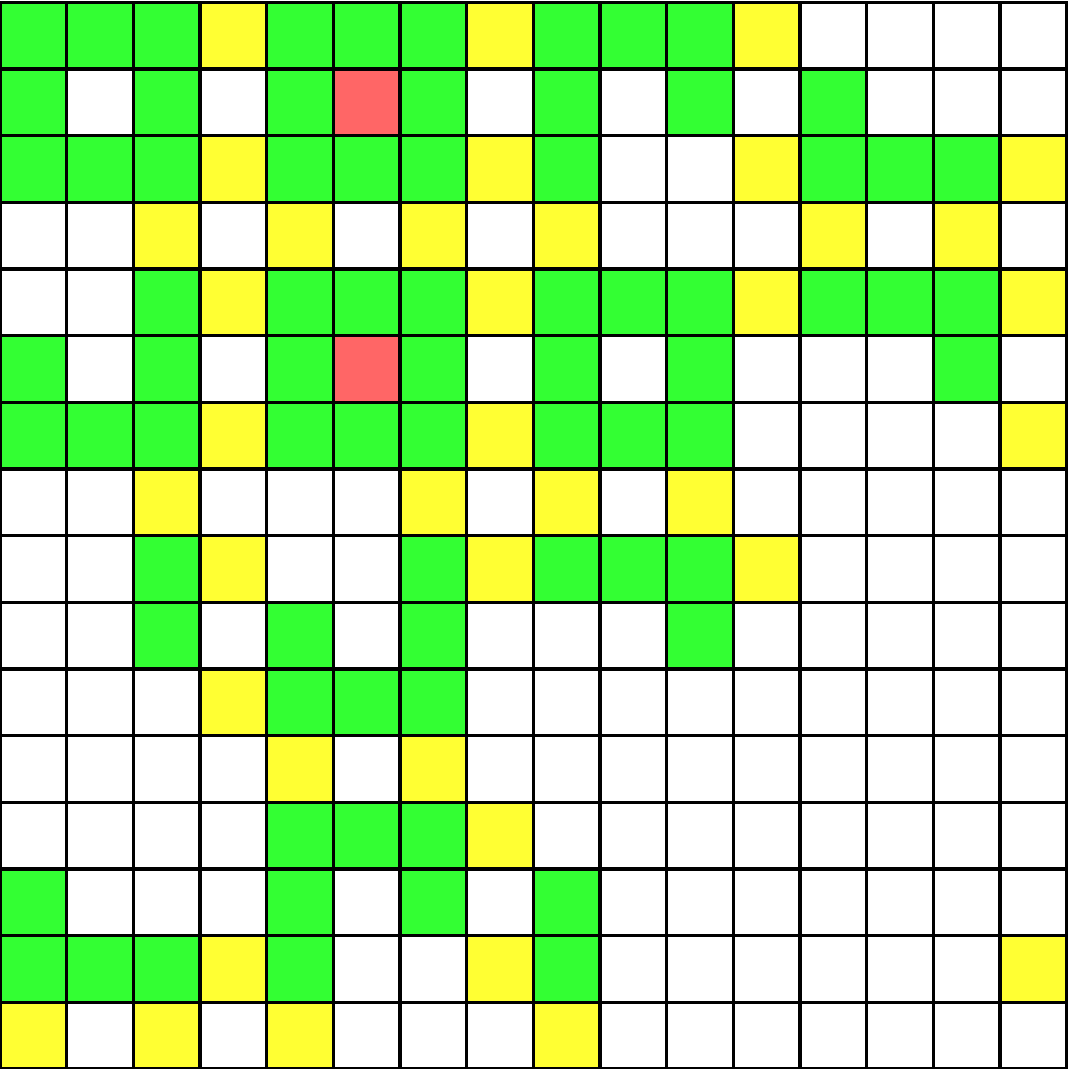
\includegraphics[width=0.9\textwidth]{replicator/11}
        \caption{Step 11}
    \end{subfigure}
\end{figure}

\begin{figure}[!ht]
    \ContinuedFloat
    \centering
    \begin{subfigure}{0.32\textwidth}
        \centering
        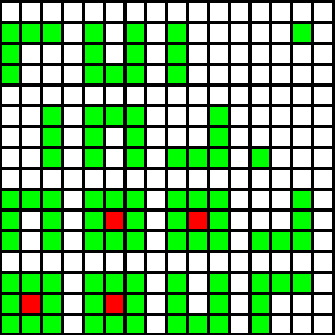
\includegraphics[width=0.9\textwidth]{replicator/12}
        \caption{Step 12}
    \end{subfigure}
    \begin{subfigure}{0.32\textwidth}
        \centering
        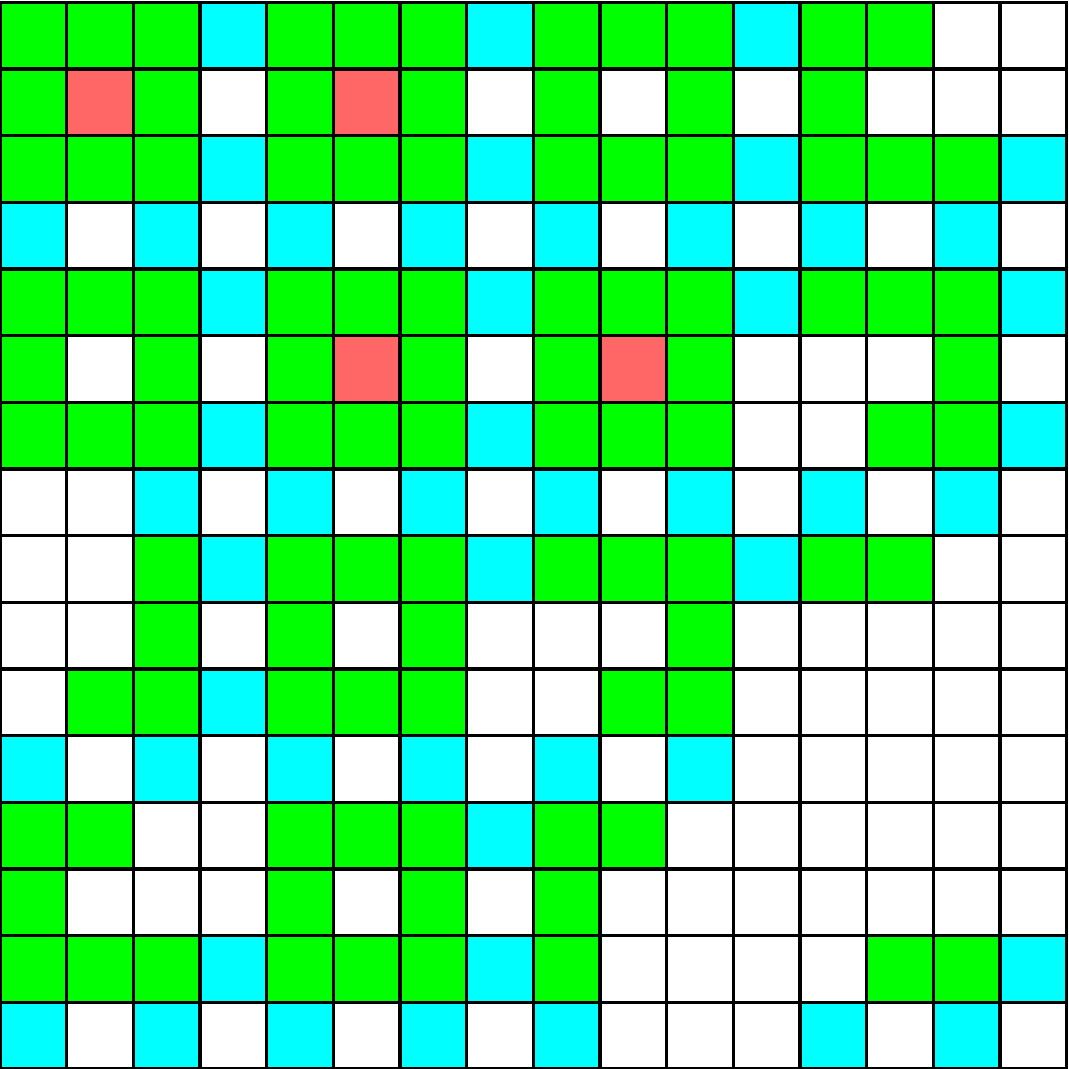
\includegraphics[width=0.9\textwidth]{replicator/13}
        \caption{Step 13}
    \end{subfigure}
    \begin{subfigure}{0.32\textwidth}
        \centering
        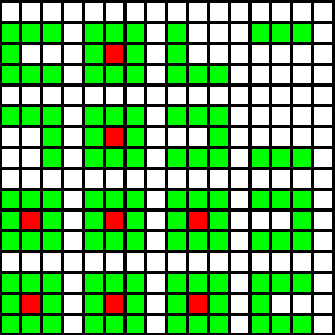
\includegraphics[width=0.9\textwidth]{replicator/14}
        \caption{Step 14}
    \end{subfigure}
    \par\bigskip
    \begin{subfigure}{0.32\textwidth}
        \centering
        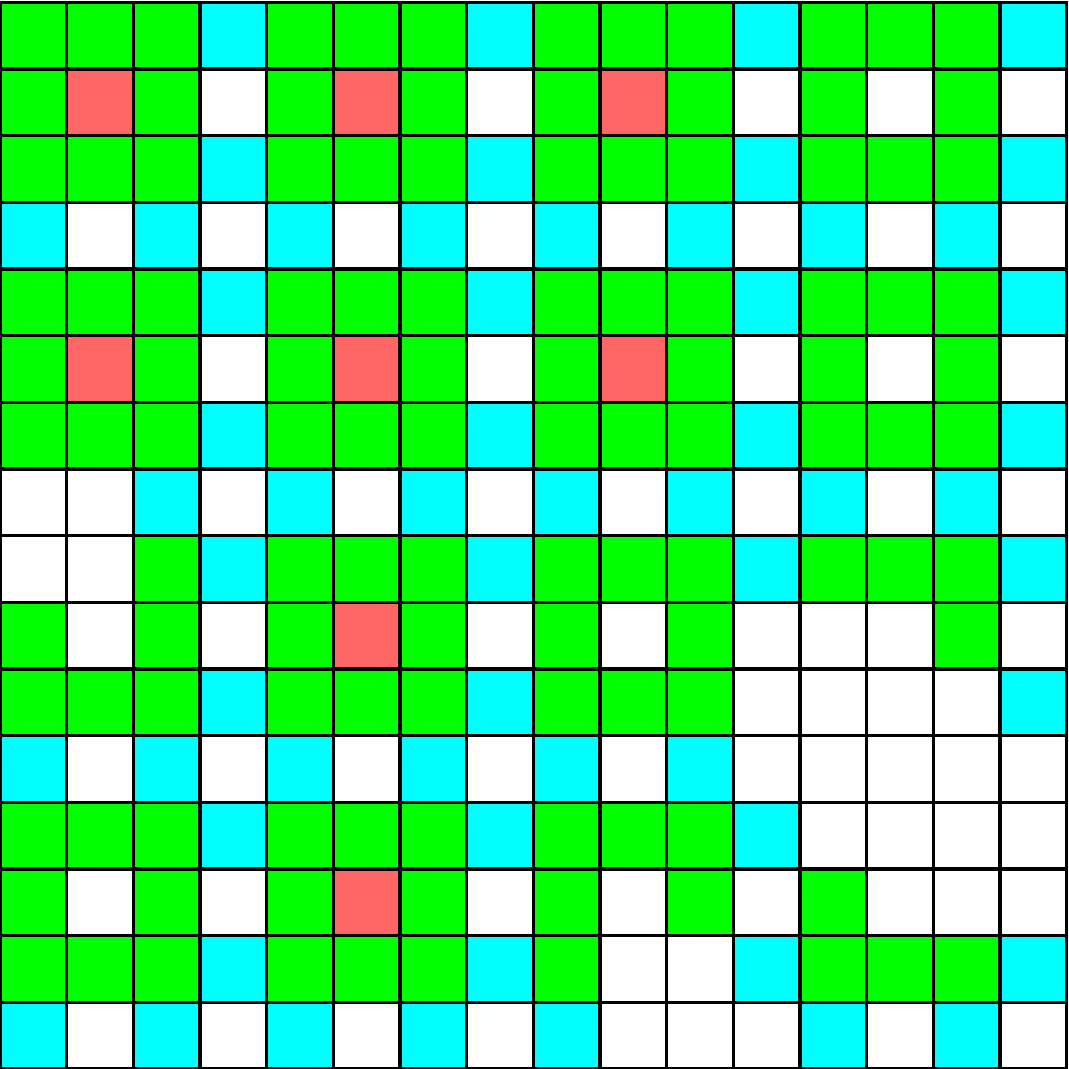
\includegraphics[width=0.9\textwidth]{replicator/15}
        \caption{Step 15}
    \end{subfigure}
    \begin{subfigure}{0.32\textwidth}
        \centering
        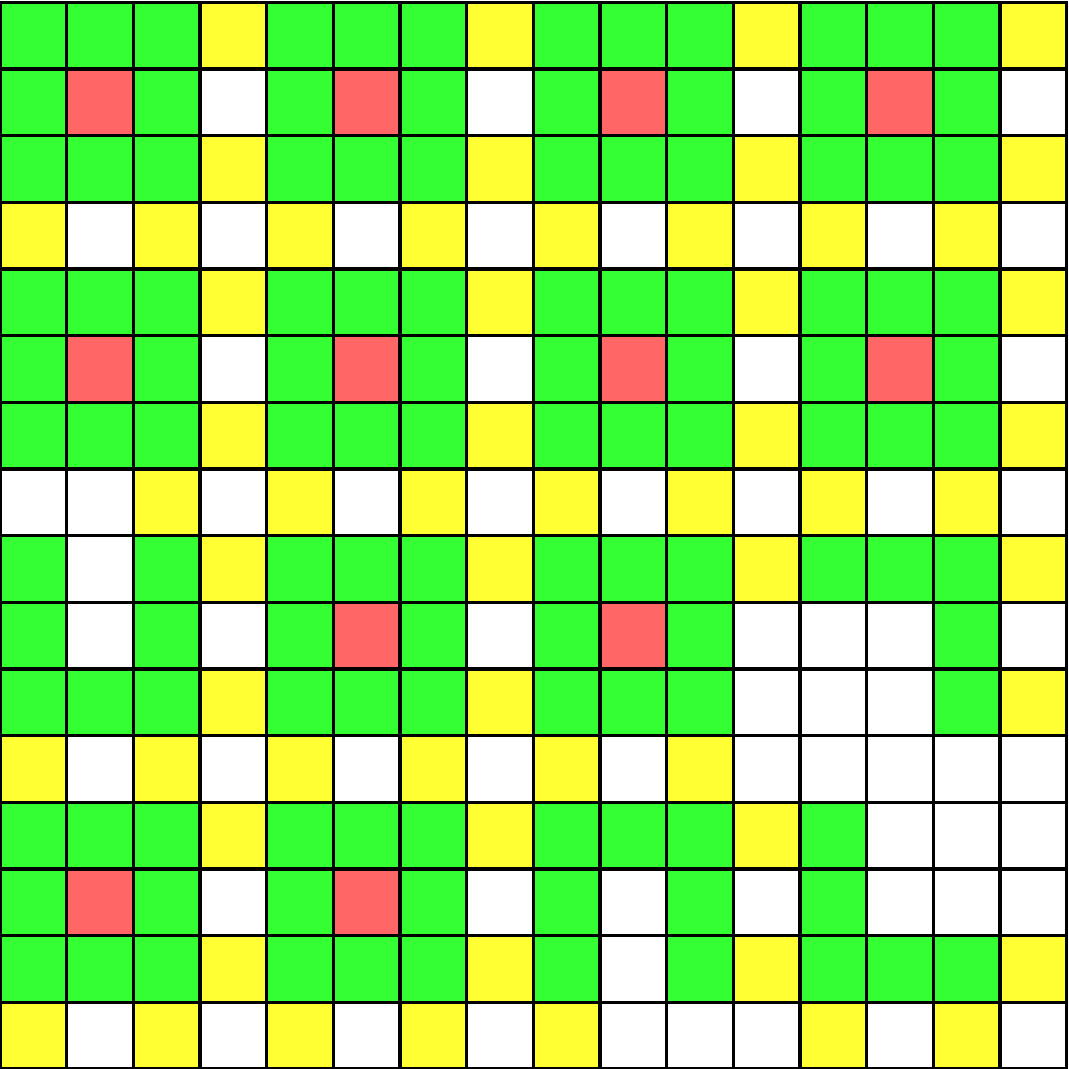
\includegraphics[width=0.9\textwidth]{replicator/16}
        \caption{Step 16}
    \end{subfigure}
    \begin{subfigure}{0.32\textwidth}
        \centering
        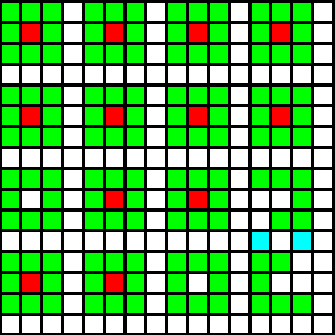
\includegraphics[width=0.9\textwidth]{replicator/17}
        \caption{Step 17}
    \end{subfigure}
    \par\bigskip
    \begin{subfigure}{0.32\textwidth}
        \centering
        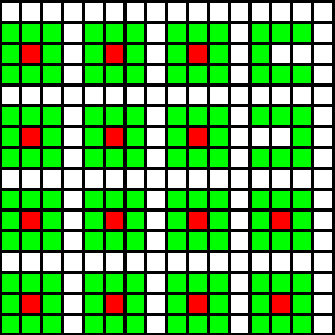
\includegraphics[width=0.9\textwidth]{replicator/18}
        \caption{Step 18}
    \end{subfigure}
    \begin{subfigure}{0.32\textwidth}
        \centering
        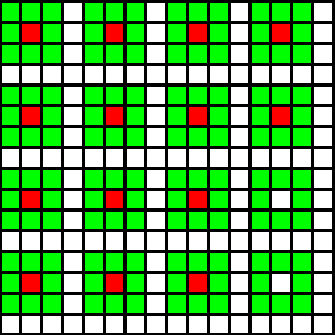
\includegraphics[width=0.9\textwidth]{replicator/19}
        \caption{Step 19}
    \end{subfigure}
    \begin{subfigure}{0.32\textwidth}
        \centering
        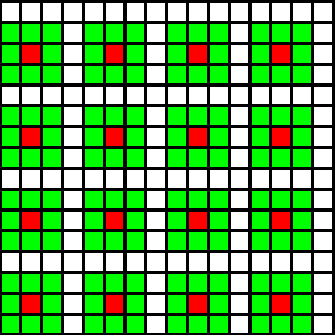
\includegraphics[width=0.9\textwidth]{replicator/20}
        \caption{Step 20}
    \end{subfigure}
    \caption[Replicator] {
        Simple 2D replicator.
        The images are created using the PostScript API.
    }
    \label{fig:replicator}
\end{figure}
